\documentclass{article}
\usepackage{amsmath} % for advanced math environments
\usepackage{amsfonts} % for math fonts
\usepackage{amssymb} % for math symbols
\usepackage{amsthm} % for theorems and proofs
\usepackage{mathtools} % for mathematical tools
\usepackage{mathrsfs} % for script-like fonts in math
\usepackage{bm} % for bold math symbols
\usepackage{bbm} % for "blackboard-style" characters in math
\usepackage{graphicx} % for including graphics
\usepackage{hyperref} % for including hyperlinks
\usepackage{tcolorbox}
\usepackage{tikz}
\tcbuselibrary{theorems, breakable}
\usepackage{xcolor}
\usepackage[margin=1in]{geometry}

\newcommand{\C}{\mathbb{C}}
\newcommand{\N}{\mathbb{N}}
\newcommand{\Q}{\mathbb{Q}}
\newcommand{\R}{\mathbb{R}}
\newcommand{\Z}{\mathbb{Z}}
\newcommand{\pset}{\mathscr{P}}
\DeclareMathOperator{\lcm}{lcm}

% Define a shortcut for \begin{bmatrix} and \end{bmatrix}
\newcommand{\bmat}[1]{\begin{bmatrix}#1\end{bmatrix}}
\newcommand{\cmat}[1]{\begin{pmatrix}#1\end{pmatrix}}

\newtcolorbox[auto counter]{problem}%
{
    breakable,
    colback=cyan!5,
    colframe=cyan!35!black,
    fonttitle=\bfseries,
    title=Problem~\thetcbcounter,
}

\newtcolorbox{solution}[1]
{
    breakable,
    colback=red!5,
    colframe=red!75!black,
    fonttitle=\bfseries,
    title=Solution: #1,
}

% Title
\title{Your Document Title}
\author{Your Name}
\date{\today} % or specify a date like {December 2020}

\begin{document}

\maketitle

\begin{problem}
Let $A = \{0, 1, 2, 3, 4, 5\}$. Write out the relation $R$ that expresses $ > $ on $A$. Then illustrate it with a diagram.
\end{problem}

Include all the ordered pairs where the first coordinate is strictly greater than the second coordinate:
$$R = \{(1, 0), (2, 1), (2, 0), (3, 2), (3, 1), (3, 0), \ldots , (5, 1), (5, 0)\}$$
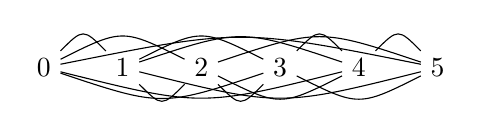
\begin{tikzpicture}
  \node (0) at (0,0) {0};
  \node (1) at (1,0) {1};
  \node (2) at (2,0) {2};
  \node (3) at (3,0) {3};
  \node (4) at (4,0) {4};
  \node (5) at (5,0) {5};

  % Draw edges
  \draw (1) .. controls (0.5,0.5) .. (0); % above
  \draw (2) .. controls (1.5,-0.5) .. (1); % below
  \draw (2) .. controls (1,0.5) .. (0); % above
  \draw (3) .. controls (2.5,-0.5) .. (2); % below
  \draw (3) .. controls (2,0.5) .. (1); % above
  \draw (3) .. controls (1.5,-0.5) .. (0); % below
  \draw (4) .. controls (3.5,0.5) .. (3); % above
  \draw (4) .. controls (3,-0.5) .. (2); % below
  \draw (4) .. controls (2.5,0.5) .. (1); % above
  \draw (4) .. controls (2,-0.5) .. (0); % below
  \draw (5) .. controls (4.5,0.5) .. (4); % above
  \draw (5) .. controls (4,-0.5) .. (3); % below
  \draw (5) .. controls (3.5,0.5) .. (2); % above
  \draw (5) .. controls (3,-0.5) .. (1); % below
  \draw (5) .. controls (2.5,0.5) .. (0); % above
\end{tikzpicture}

\begin{problem}
Let $A = \{1, 2, 3, 4, 5, 6\}$. Write out the relation $R$ that expresses $\mid$ (divides) on $A$. Then illustrate it with a diagram.
\end{problem}

First note that 1 divides everything, so $(1, x)$ will be in $R$ for all $x \in A$. 2 divides itself, 4, and 6, 3 divides itself and 6, and the rest only divide themselves:
$$R = \{(1, 1), (1, 2), \ldots, (1, 6), (2, 2), (2, 4), (2, 6), (3, 3), (3, 6), (4, 4), (5, 5), (6, 6)\}$$

\begin{problem}
Let $A = \{0, 1, 2, 3, 4, 5\}$. Write out the relation $R$ that expresses $\geq$ on $A$. Then illustrate it with a diagram.
\end{problem}

$$R = \{(0, 0), (1, 1), (1, 0), (2, 2), (2, 1), (2, 0), \ldots, (5, 1), (5, 0)\}$$

\begin{problem}
Here is a diagram for a relation $R$ on a set $A$. Write the sets $A$ and $R$.
\end{problem}
\begin{figure}[h]
  \centering
  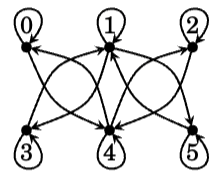
\includegraphics[width=0.5\textwidth]{11.4.png}
  \label{fig:example}
\end{figure}

The set $A$ are the letters 0 through 5. We see that relation is reflexive and symmetric but not transitive. It appears to be similar to the 'same parity' relation but missing some elements.
$$R = \{(0, 0), (1, 1), \ldots, (5, 5), (0, 4), (4, 0), (1, 3), (3, 1), (2, 4), (4, 2), (1, 5), (5, 1)\}$$

\begin{problem}
Here is a diagram for a relation $R$ on a set $A$. Write the sets $A$ and $R$.
\end{problem}

\begin{figure}[h]
  \centering
  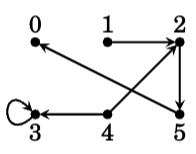
\includegraphics[width=0.5\textwidth]{11.5.png}
  \label{fig:example}
\end{figure}

The set $A$ are the nodes on the graph:
$$A = \{0, 1, 2, 3, 4, 5\}$$

The set $R$ is the ordered pairs for the arrows:
$$R = \{(1, 2), (2, 5), (3, 3), (4, 2), (4, 3), (5, 0)\}$$

\begin{problem}
Congruence modulo 5 is a relation on the set $\Z$. In this relation $xRy$ means $x \equiv y \pmod{5}$. Write out the set $R$ in set-builder notation.
\end{problem}

Elements of $R$ are ordered pairs $(x, y)$, since $R \subseteq \Z \times \Z$. We also need to specify that a pair $(x, y)$ belongs to $R$ only if $x$ and $y$ are congruent mod 5:
$$R = \{(x,y) \in \Z^2 \mid x \equiv y \pmod{5}\}$$

\begin{problem}
Write the relation < on the set $\Z$ as a subset $R$ of $\Z \times Z$. This is an infinite set, so you will have to use set builder notation.
\end{problem}

$$R = \{(x, y) \in \Z^2 \mid x < y\}$$

\begin{problem}
Let $A = \{1, 2, 3, 4, 5, 6\}$. Observe that $\varnothing \subseteq A \times A$, so $R = \varnothing$ is a relation on $A$. Draw a diagram for this relation.
\end{problem}

The diagram would be a graph with nodes 1 through 6, no edges (since there are no relationships in the set).

\begin{problem}
Let $A = \{1, 2, 3, 4, 5, 6\}$. How many different relations are there on the set $A$?
\end{problem}

Any subset of $A \times A$ qualifies as a relation, so the answer will be $|\mathcal{P}(A \times A)|$. Since $|A| = 6$ the product $|A \times A| = 36$, and $|\mathcal{P}(A \times A)| = 2^{36}$.

\begin{problem}
Consider the subset $R = (\R \times \R) - \{(x, x) : x \in \R\} \subseteq \R \times \R$. What familiar relation on $\R$ is this? Explain.
\end{problem}

The relation $R$ starts with all ordered pairs in $\R^2$ but then removes the pairs with the same value on both coordinates. So every real number has this relationship to every other real number but not itself. That's the $\neq$ relation.

\begin{problem}
Given a finite set $A$, how many different relations are there on $A$?
\end{problem}

As we saw in a previous problem, it's the number of subsets the product $A \times A$ has: $|\mathcal{P}(A \times A)|$.


\end{document}
